Certainly! Below is an example of a universal quantum ansatz function \(\hat{U}({\bm \lambda})\) for \(n = 3\) qubits using parameterized \(R_y(\lambda_i)\) rotations and CNOT gates in TikZ LaTeX.

```latex
\documentclass{standalone}
\usepackage{tikz}

\begin{document}

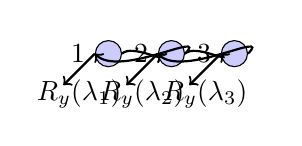
\begin{tikzpicture}[x=1cm, y=1cm, scale=0.8]
    % Qubits
    \node[circle, draw, fill=blue!20] (q1) at (0,0) {};
    \node[circle, draw, fill=blue!20] (q2) at (1,0) {};
    \node[circle, draw, fill=blue!20] (q3) at (2,0) {};

    % R_y Gates
    \draw[->, thick] (q1.west) -- ++(-0.5,-0.5) node[midway, below] {$R_y(\lambda_1)$};
    \draw[->, thick] (q2.west) -- ++(-0.5,-0.5) node[midway, below] {$R_y(\lambda_2)$};
    \draw[->, thick] (q3.west) -- ++(-0.5,-0.5) node[midway, below] {$R_y(\lambda_3)$};

    % CNOT Gates
    \draw[thick, ->] (q1.east) to[out=45,in=-45] (q2.west);
    \draw[thick, ->] (q2.east) to[out=45,in=-45] (q3.west);

    % Additional CNOT Gates
    \draw[thick, ->] (q2.east) to[out=45,in=-45] (q1.west);
    \draw[thick, ->] (q3.east) to[out=45,in=-45] (q2.west);

    % Labels
    \node[left] at (q1.west) {1};
    \node[left] at (q2.west) {2};
    \node[left] at (q3.west) {3};
\end{tikzpicture}

\end{document}
``